\documentclass[12pt, 
openright, 
oneside, 
%twoside, %TCC: Se seu texto tem mais de 100 páginas, descomente esta linha e comente a anterior
a4paper,    
%english,   
brazil]{facom-ufu-abntex2}



\autor{Igor Batista Fernandes} 
\data{2018}
\orientador{Profa. Maria Adriana Vidigal de Lima} 
\titulo{Desenvolvimento de jogos 2D multiplataforma utilizando
OpenGL e Java} 

\begin{document}
\pagenumbering{arabic}
% ----------------------------------------------------------
% ELEMENTOS PRÉ-TEXTUAIS

\imprimircapa
\begin{folhadeaprovacao}

  \begin{center}
    {\ABNTEXchapterfont\large\imprimirautor}

    \vspace*{\fill}\vspace*{\fill}
    {\ABNTEXchapterfont\bfseries\Large\imprimirtitulo}
    \vspace*{\fill}
    
    \hspace{.45\textwidth}
    \begin{minipage}{.5\textwidth}
    \imprimirpreambulo
    \end{minipage}%
    \vspace*{\fill}
   \end{center}
    
   %Trabalho aprovado. 
   \imprimirlocal, XX de XX de 2018: %TCC:

   \assinatura{\textbf{\imprimirorientador} \\ Orientador}  
   \assinatura{\textbf{Professor}}% \\ Convidado 1} %TCC:
   \assinatura{\textbf{Professor}}% \\ Convidado 2} %TCC:
   %\assinatura{\textbf{Professor} \\ Convidado 3}
   %\assinatura{\textbf{Professor} \\ Convidado 4}
      
   \begin{center}
    \vspace*{0.5cm}
    {\large\imprimirlocal}
    \par
    {\large\imprimirdata}
    \vspace*{1cm}
  \end{center}
  
\end{folhadeaprovacao}
%-------------------------------------------
% RESUMO

\begin{resumo} 

Este trabalho propõe a criação de um jogo multiplataforma  para desktop intitulado Traveller.
A elicitação dos requisitos para a elaboração do jogo será documentada em um artefato denominado \textit{Game Design Document} que permite estruturar, sistematizar e organizar 
o processo de construção do jogo.
A implementação de código será realizada na linguagem Java e através da API gráfica OpenGL usando GLFW (OpenGL Frame Work). 
O jogo será elaborado utilizando-se algoritmos procedurais para geração de algumas artes e ambientes, algoritmos genéticos para o comportamento de Non Playable Characters (NPC) e padrões de projeto como o MVC.
 
 \vspace{\onelineskip}
 \noindent
 \textbf{Palavras-chave}: Indie Game, Game Design Document, Jogos, Java, OpenGL
\end{resumo}

\begin{abstract} 
This work proposes to develop a multiplataform game for desktop entitled Traveller. The elicitation of requisites for the game will be documented in an artifact called Game Design Document which allows to structure, systematize and organize the process of building a game. The code implementation will be done in Java through the API OpenGL and GLFW.  The game will be elaboreted using procedural algorithms to generate some art and environment, genetic algorithms for NPC behaviours and design patterns such as MVC.

 \vspace{\onelineskip}
    
 \noindent
 \textbf{Keywords}: Indie Game, Game Design Document, Games, Java, OpenGL %TCC:
\end{abstract}
\cleardoublepage

% ------------------------------------------
% LISTA DE FIGURAS

\pdfbookmark[0]{\listfigurename}{lof}
\listoffigures*
\cleardoublepage

% ------------------------------------------
% LISTA DE TABELAS

\pdfbookmark[0]{\listtablename}{lot}
\listoftables*
\cleardoublepage

% ------------------------------------------
% LISTA DE CÓDIGOS
\pdfbookmark[0]{\listtablename}{lol}
\lstlistoflistings
\cleardoublepage

% ------------------------------------------
% LISTA DE ABREVIATURAS OU SIGLAS

\begin{siglas} 
  \item[GDD] Game Design Document 
  \item[API] Application Programming Interface
  \item[MVC] Model-view-controller
  \item[OpenGL] Open Graphics Library
  \item[GPU] Graphics Processing Unit
  \item[GLFW] Graphics Library Framework
  \item[GLSL] OpenGL Shading Language
  \item[NPC] Non Playable Character
  \item[HUD] Heads-Up Display
  \item[ASD] A Ser Definido
  \item[FPS] Frames per second
  \item[px] Pixel (Unidade de medida)
  \item[VBO] Vertex Buffer Object
  \item[VAO] Vertex Array Object
\end{siglas}


% SUMÁRIO
% ---
\pdfbookmark[0]{\contentsname}{toc}
\tableofcontents*
\cleardoublepage


% ------------------------------------------
% COMEÇAR O TEXTO

%\textual

% ------------------------------------------% INTRODUÇÃO

% colocar como subitem 
%\chapter*[Introdução]{Introdução}
%\addcontentsline{toc}{chapter}{Introdução}

\chapter{Introdução}

\section{Visão Geral da Proposta}
O mercado internacional de jogos movimentará aproximadamente 108.9
bilhões de dólares distribuídos entre 2.2 bilhões de jogadores. Destes, 58\%
representam os segmentos de PC e consoles \cite{GameMarketArticle}. Além de ser uma área
comercial extremamente lucrativa é também interdisciplinar e aproxima
conceitos de Computação, Design gráfico, Música, Artes e outras esferas do
conhecimento.
Para a elaboração de um projeto bem construído e com alto potencial de
sucesso é necessário respeitar as etapas de pré-produção, produção, testes
e pós-produção. Ao longo de todas as etapas serão definidas estratégias de
implementação em linguagens orientadas a objetos, Engenharia de software
voltada par jogos e metodologias ágeis.
Desenvolvida pela Khronos Group a API OpenGL fornece tudo que há de mais
avançado em aplicações gráficas, sendo acelerada diretamente em
hardware, multiplataforma, robusta e totalmente escalável.


%Objetivo
\section{Objetivo}
O objetivo é desenvolver um jogo seguindo a construção de um Game Design
Document (GDD) e ter o produto final publicado e distribuído
comercialmente de maneira digital. Ao final deste documento será
apresentada a primeira fase do capítulo introdutório, jogável e com
qualidade profissional.

\section{Justificativa e Motivação}
O consumo cada vez maior deste tipo de produto pela população de todas as idades traz cada vez mais oportunidades de trabalho e aprendizagem.
A insuficiência de materiais em língua portuguesa sobre os processos de desenvolvimento e planejamento de jogos é um grande instigador desse trabalho. Neste contexto, esse trabalho aborda todas as etapas pelas quais um jogo passa para torna-se um software que será distribuído e jogado por pessoas do mundo todo.


\section{Metodologia}


Este trabalho se classifica como uma pesquisa aplicada, sendo o método de desenvolvimento baseado nas etapas a seguir:

Etapa 1 – Revisão sistemática em desenvolvimento de jogos
\begin{itemize}
\item Desenvolvimento de Jogos estilo RPG - levantamento bibliográfico, identificação e organização dos trabalhos relacionados e do estado da arte;
\item Pesquisa documental sobre engenharia de software e padrões de projeto aplicada a jogos;
\item Pesquisa documental sobre o uso de metodologias ágeis no desenvolvimento de jogos.
\end{itemize}

Etapa 2 – Projeto do jogo identificando os conceitos a serem aplicados 
\begin{enumerate}
\item Pré-Projeto: análise de mercado, tendências e viabilidade;
definição da ideia do seu jogo; atividades a serem realizadas;
equipe.
\item Pré-Produção: elaboração do Game Design Document, elaboração do Roteiro, elaboração do Documento de Arte e Design Gráfico; criação de protótipos para testar ideias, mecânicas e conceitos;
\item Plano de Produção: criação de um cronograma e planejamento dos ciclos de trabalho da produção, considerando o desenvolvimento do jogo utilizando uma  metodologia ágil (SCRUM). Desenvolvimento de uma game engine/framework para a construção do jogo. Análise de requisitos do jogo. Os requisitos serão documentados usando diagramas de casos de uso em paralelo ao uso do GDD.
\end{enumerate}

Etapa 3 – Implementação do jogo em formato digital. O desenvolvimento será dividido nos seguintes ciclos:
\begin{enumerate}
\item Desenvolvimento e testes de unidade do módulo gráfico
(cenários, animações, mecânica).
\item Desenvolvimento e testes de unidade do módulo de físicas
(colisões em geral).
\item Desenvolvimento e teste de unidade do módulo de áudio.
\item Desenvolvimento de interfaces e ferramentas.
\item Desenvolvimento das artes e teste de fluxo.
\item Teste de sistema e ajustes.
\end{enumerate}
Etapa 4 – Testes e avaliação do jogo.
\begin{enumerate}
\item Etapa alfa. Consiste de um período de testes com um grupo seleto de pessoas.
\item Etapa Beta. Etapa de testes aberta e já próxima do lançamento final.
\item Lançamento.
\end{enumerate}

\section{Cronograma}
O cronograma é apresentado segundo formatos e exemplos do livro Manual de produções de jogos digitais \cite{Manualdejogosdigitais}:
\begin{figure}[!htb]
	\centering
	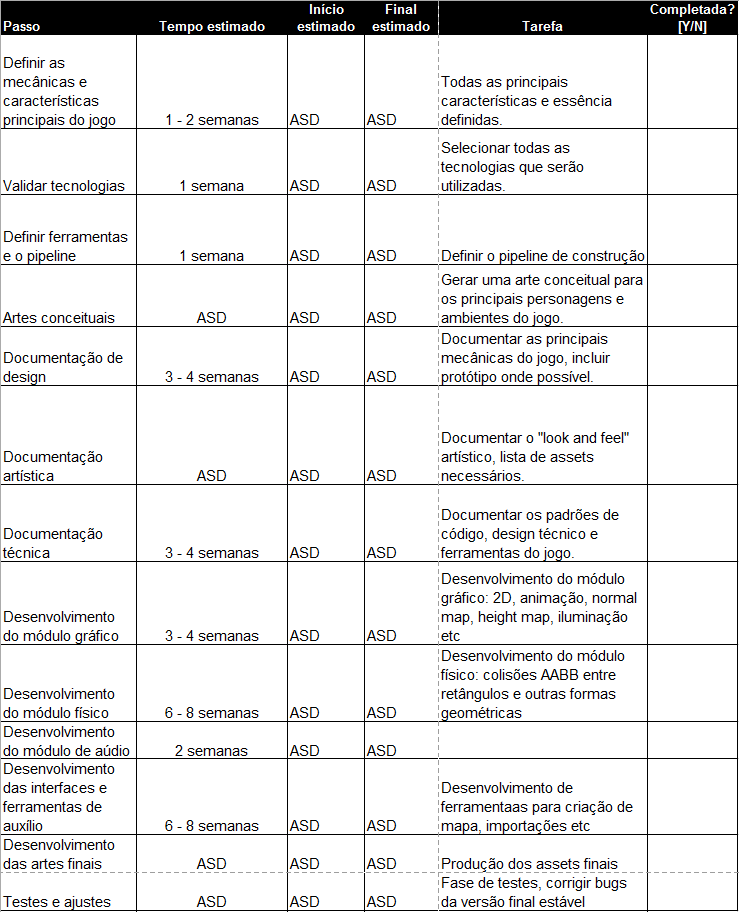
\includegraphics[width=4in]{imagens/cronograma.png}
	\caption{Tabela com uma estimativa de tempo para cada passo do desenvolvimento}
\end{figure}

% ------------------------------------------
% REFERENCIAL TEÓRICO

\chapter{Revisão Bibliográfica}

\section{Referencial Teórico}
\label{sec:refteo}
\subsection{OpenGL}
A API (Application Programming Interface) OpenGL fornece um conjunto de funções para manipulações gráficas \cite{LearnOpenGL}, sendo acelerada diretamente em hardware, multiplataforma, robusta e totalmente escalável. Embora comumente referida como uma API, o OpenGL é, por si só, um conjunto de especificações que determinam o resultado/saída de cada função e como devem ser executadas. Fica a cargo dos manufaturadores de placas gráficas implementarem a operação da função, respeitando as especificações do documento desenvolvido e mantido pela Khronos Group \cite{KhronosOpenGLSpecification}.
 O OpenGL foi lançado em 1992 como uma resposta direta a necessidade de se padronizar o conjunto de instruções usado em hardwares com interface gráfica. Até setembro de 2006 o padrão foi mantido pela ARB (Architecture Review Board), um conselho formado por empresas de grande renome no ramo como HP, IBM, Intel, NVIDIA, Dell e a própria fundadora, a Silicon Graphics. Em setembro de 2006 o conselho ARB tornou-se o OpenGL Working Group gerido e mantido pelo consórcio Khronos Group para Open Standard APIs\cite{OpenGLAbout}.
 
\subsection{Engenharia de software}
A engenharia de software em um jogo, para ser bem sucedida, precisa respeitar as etapas de pré-produção, produção, testes (ou Quality Assurance) e pós-produção [Manual de produção de jogos digitais – Pg. 3]. A metodologia de desenvolvimento a ser utilizada neste trabalho será o SCRUM.

\subsection{Pré-Produção}
A etapa de pré-produção é crítica e determina como será o jogo, quanto tempo levará o desenvolvimento, quantas pessoas serão necessárias e quanto irá custar tudo. Geralmente consome de 10 a 25\% do tempo total do desenvolvimento \cite{Manualdejogosdigitais}. É nessa etapa que se elabora o Game Design Document (GDD) contendo todo o conceito do jogo e requisitos do projeto.

\subsection{Produção}
Durante a produção será elaborado os assets e código do jogo. É nela que ocorrem a criação do conteúdo propriamente dito e o rastreamento do progresso e conclusão de tarefas\cite{Manualdejogosdigitais}. Para equipes pequenas é interessante metodologias ágeis que focam na produção invés de documentação.

\subsection{Testes}
Em jogos há duas grandes fases para verificar se tudo está funcionando como o esperado: Alfa e Beta. Durante todo o processo é necessário uma equipe do Departamento de Qualidade verificando bugs e reportando-os. Entretanto, as fases Alfa e Beta são as mais importantes. A fase alfa é quando uma seleta quantidade de usuários é escolhida para testar o jogo e dar feedback à desenvolvedora. Ela é fundamental para garantir que o jogo funciona como esperado e quais aspectos precisam ser melhorados antes de ser distribuída para o público geral. A etapa seguinte, Beta, é geralmente aberta ao público e já possui boa parte dos bugs corrigidos. Ela é essencial para testar a recepção do público e fazer as correções finais antes do lançamento oficial.

\subsection{Game Design Document}
Como em todo software o jogo também possui um documento de requisitos. Entretanto, um documento de requisitos não é suficiente para detalhar todos os elementos que compõe um jogo.  Essa carência de especificações como história, personagens, roteiro, câmera entre outras coisas são supridas pelo GDD.  Portanto, no caso especial de um jogo é necessário ambos documentos para detalhar e especificar adequadamente o projeto. Entretanto, não há regra universal ou normas que ditem como exatamente um GDD deve ser construído ou quais conteúdos deve abranger. A estrutura de um GDD é, possivelmente, composta dos seguintes itens \cite{LevelUp}:\\ %TODO: Citei apenas os mais relevates, isso altera a maneira de citar uma vez que não está idêntico ao do livro?
\textbf{Objetivos de jogo} – Detalha o conceito geral do jogo.\\
\textbf{Visão geral da história} – Constitui um breve resumo da história. Deve entrelaçar os diversos elementos narrativos como ambientes e personagens e conter o início, meio e fim da narrativa. \\
\textbf{Controles do jogo} – Lista de movimentos que o jogador poderá realizar como ataques, rolamento e corrida. Deve mapear cada botão do controle com a ação a ser realizada. \\
\textbf{Exigências de tecnologia} – Ferramentas que serão utilizadas ou implementadas para design de níveis, câmeras, engine, física etc. \\
\textbf{Front end do jogo} – Indica quais telas de crédito serão mostradas quando o jogo é ligado pela primeira vez incluindo: 
	\begin{itemize}
	\item Distribuidor
	\item Logo do estúdio
	\item Licenciadores
	\item Produtores de software terceirizados
	\item Tela com legislação
	\end{itemize}
\textbf{Tela de título/início} - Deve conter em detalhes o que é apresentado ao jogador nas telas iniciais, de preferência com imagens, como por exemplo: Título e como ele aparece na tela, tela de configurações (vídeo, áudio, música, subtítulos etc.), lista de detalhes dos arquivos salvos etc.\\
\textbf{Outras telas} - Todas as outras telas que não as de início. Por exemplo: Créditos, Conteúdos desbloqueáveis, easter eggs, roupas e armas alternativas etc.\\
\textbf{Fluxo de jogo} - Demonstra através de um fluxograma como todas as telas interagem entre si.\\
\textbf{Câmeras(s) de jogo} - Deve conter todos os tipos de câmeras utilizadas, sejam primeira pessoa, terceira pessoal, de rolagem etc.\\
\textbf{Sistema de HUD} - Informações apresentadas em tela para o jogador. Deve conter imagens demonstrados aspectos como: Saúde, Vidas, Dinheiro, Mini Mapa, Sistema de mira, Sistema de navegação, habilidades etc.\\
\textbf{Personagem do jogador} - Alguns conceitos visuais e textuais de quem é o personagem que o jogador irá controlar.\\
\textbf{Métricas do jogador} - Relações de tamanho do personagem do jogador com outros/elementos no mundo:
	\begin{itemize}
	\item Movimento (caminhada, corrida, movimento furtivo, mergulho,rolagem, rastejada)
	\item Navegação (nado, pulo, voo)
	\item Pendurar/Balançar
	\item Movimentos sensíveis ao contexto (empurrar/puxar, iterações com objetos etc.)
	\item Reações/danos/morte	
	\end{itemize}
\textbf{Habilidades do jogador} - Descrição de cada uma das habilidades e seus upgrades, modificadores e métricas.
\textbf{Mecânicas Universais de jogo} - Descrição breve de como cada uma das mecânicas que compõe o jogo funciona.
\textbf{Pontuação} - Métricas de como o jogador é recompensado. Placares de liderança e  Achievements.
\textbf{Economia} - Sistema monetário e o que é possível obter com a moeda. Lista custos.
\textbf{Veículos} - Como funcionam os veículos. Como interagir, suas métricas e controles.
\textbf{Personagens relevantes na história} - Um breve resumo de cada personagem importante para a história e o seu papel. Mostrar imagens.
\textbf{Esboço da progressão do jogo} - Mostrar em um esboço textual ou visual como seria jogar o jogo do começo ao fim. Deixe explicito como o jogador é recompensado conforme progride na história.   
\textbf{Regras gerais dos inimigos} - Listar:
	\begin{itemize}
	\item Tipos de comportamento (patrulheiro, caçador etc.)
	\item Regras de IA e métricas de detecção
	\item Parâmetros de nascimento
	\item Parâmetros de derrota etc.
	\end{itemize}
\textbf{Personagens não jogáveis (NPCs)} - Descrição breve dos tipos de NPC e listar possíveis características como nomes, onde encontrá-los, história etc. Determinar também as interações possíveis.\\
\textbf{MiniGames} - Lista quais minigames estão presentes bem como seus controles e onde aparecem.\\
\textbf{Cenas de corte} - Listar as cenas de corte.\\
\textbf{Músicas e efeitos especiais} - Listar as músicas e efeitos juntamente com seu tom/clima e onde aparecem.\\
\textbf{Apêndices} - Lista de animações do jogador, Lista de animações dos NPCs e inimigos, Lista dos efeitos sonoros, Lista de músicas, Roteiros etc.
% ------------------------------------------
% Trabalhos Correlatos

\chapter{Trabalhos Correlatos}
\label{sec:trabcorr}

%TODO: Inserir imagem
No Place for bravery: Jogo estilo Roguelike em pixel art. Atualmente em desenvolvimento pelo estúdio Glitch Factory situado no Distrito Federal.\\

%TODO: Inserir imagem
Eitr: Jogo estilo Action RPG inspirado em Dark souls com uma temática sombria e em pixel art. Atualmente em desenvolvimento pelo estúdio Devolver Digital.\\

%TODO: Inserir imagem
Kingdom: Jogo de plataforma feito em pixel art. \\

Moon Hunters: Action RPG em pixel art com mundo extenso e procedural, muito similar à proposta deste trabalho em alguns aspectos centrais. \\

Children of morta: Action RPG em pixel art. \\

% ------------------------------------------
% DESENVOLVIMENTO DO TRABALHO

\chapter{Arquitetura de uma \textit{Game Engine}}
Game engine (em português literal, motor de jogo) é o termo designado ao motor que está por trás de todo jogo. É neste conjunto de sistemas de simulação em tempo real que todo o ambiente do jogo é construído. As principais funcionalidades providas em uma engine são: um sistema de renderização 2D e/ou 3D, detecção e resolução de colisões, áudio, inteligência artificial e muitos outros. A partir desses elementos há várias ramificações em subsistemas com funcionalidades específicas para satisfazer as necessidades individuais de cada projeto. Uma engine se assemelha em muitas características a um sistema operacional. Ela lida com aspectos de baixo nível da máquina como a \textit{Graphic Processing Unit} (GPU) e é comumente construída utilizando-se o padrão de projeto em camadas. A Figura~\ref{fig:arquitetura}  ilustra um típico diagrama da arquitetura deste sistema e seus componentes.

Alguns exemplos muito populares de engines disponíveis no mercado são a Unity, Unreal Engine, Godot, Construct 2 entre muitas outras. Cada uma apresenta sua própria estrutura e especificidade. Algumas são voltadas para projetos 3D e 2D, outras são otimizadas especificamente para um ambiente 2D e outras 3D. Cabe ao projetista decidir qual desses produtos irá melhor atendê-lo conforme suas necessidades. Para este projeto, a engine utilizada será de desenvolvimento próprio.

\begin{figure}[H]
	\centering
	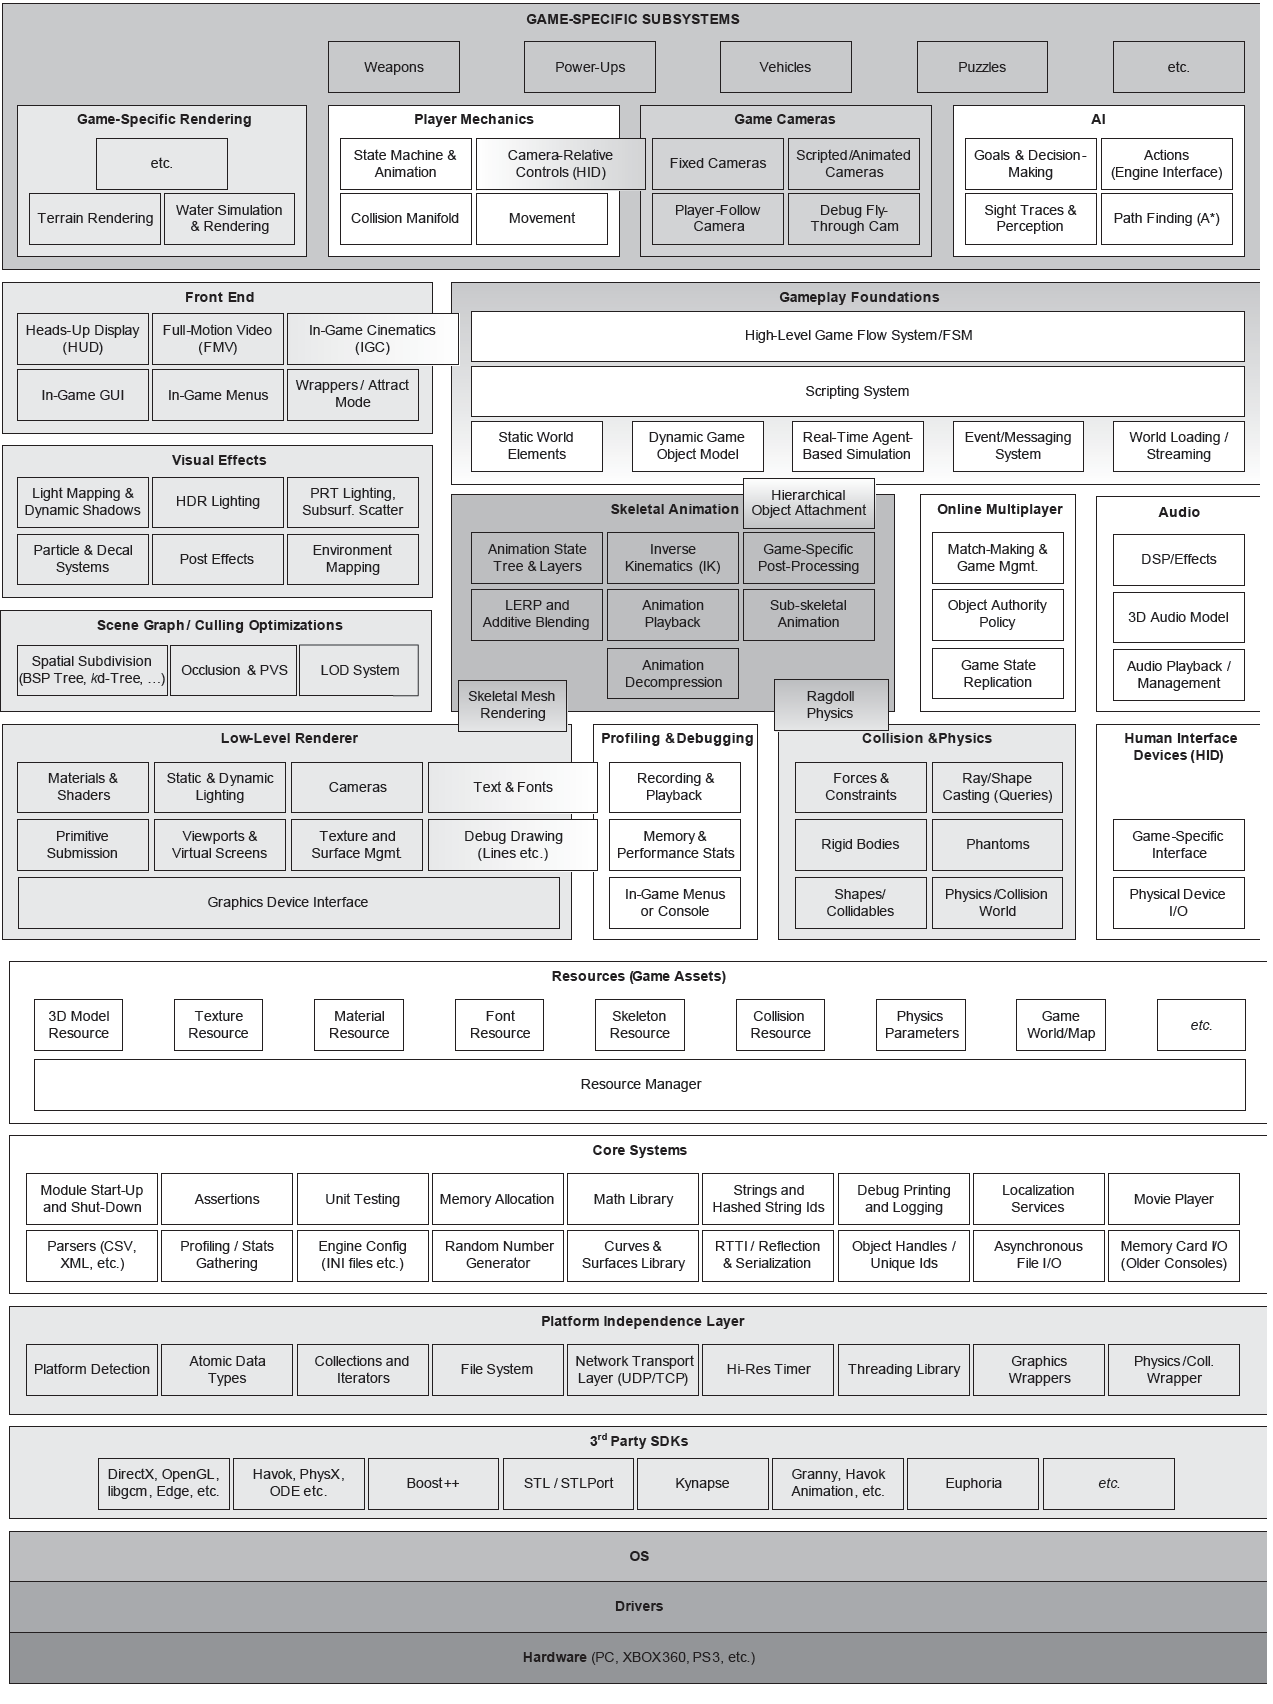
\includegraphics[width=\textwidth]{imagens/engine_layers.png}
	\caption{Componentes de uma Game Engine. Fonte:~\cite{GameEngineArchitecture}
    \label{fig:arquitetura}}
\end{figure}

\section{\textit{Game Loop}}
Game loop é o núcleo da arquitetura de uma engine. É neste loop que todos os subsistemas da engine são chamados e  executados, como a renderização, detecção e resolução de colisões, áudio e muitos outros \cite{GameEngineArchitecture}. Por se tratar de uma simulação em tempo real, onde a tela inteira deve ser atualizada em uma quantidade muito alta de vezes, é fundamental que tudo seja executado o mais rápido possível e em tempo constante para que o usuário tenha uma experiência fluída e dinâmica.

Portanto, o tempo demanda um papel chave neste sistema e deve ser cuidadosamente levado em consideração para que não haja quaisquer gargalos que deturpem a fluidez e experiência final do usuário. A estrutura mais simples de um game loop é composta como se segue:

\begin{lstlisting}[caption={Estrutura básica do Game Loop}, label={alg:gameloopbasico}]
while(true) {
	update();
	render();
}
\end{lstlisting}


O algoritmo \ref{alg:gameloopbasico} sendo executado ao longo do tempo é representado pela Figura~\ref{fig:gameloopbasico}.
Cada execução do método \texttt{render} significa o desenho de uma imagem na tela e a quantidade total de imagens desenhadas ao longo de um segundo é representada pela unidade de medida FPS (\textit{Frames per second}). Cada execução do método \texttt{update} significa um passo no tempo do jogo (\textit{timestep}). Da mesma forma que o relógio move-se em tiques de um segundo em um segundo, o tempo do jogo avança em tiques de \texttt{update} em \texttt{update}.

\begin{figure}[H]
	\centering
	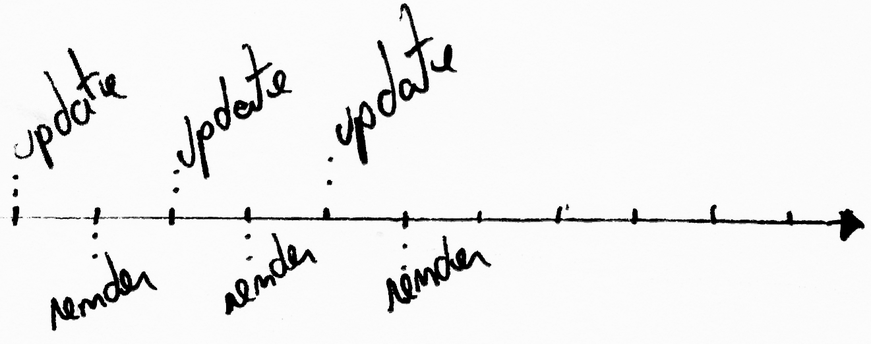
\includegraphics[width=\textwidth]{imagens/ilu1_small.png}
	\caption{Execução do game loop básico ao longo do tempo\label{fig:gameloopbasico}}
\end{figure}




\section{Sistema de atualização}
O sistema de atualização é responsável por controlar o aspecto lógico da engine. Nele ocorrem todos os cálculos relativos a movimentação dos objetos, colisões, inteligência artificial e outros. Sendo assim, é um sistema composto de outros sistemas, cada um rodando com uma taxa de atualização específica e não obrigatoriamente atrelados ao FPS.

\subsection{Timestep fixo}
Sistemas de atualização com timestep fixo são aqueles que estavam diretamente atrelados ao FPS e eram utilizados em jogos antigos \cite{GameEngineArchitecture}. As unidades de medida de tempo eram diretamente atreladas ao FPS tal que, se uma máquina fosse capaz de rodar o jogo a 30 FPS e outra a 60 FPS, na segunda máquina o jogo daria impressão de estar duas vezes mais rápido ou duas vezes mais lento dependendo do valor fixado para o timestep. Isso acontecia por que os jogos eram desenvolvidos para plataformas específicas e, sabendo em qual taxa de FPS o jogo iria rodar, era fácil delimitar um timestep fixo.

Entretanto, conforme as máquinas se tornaram mais potentes e o mercado passou a oferecer mais opções de hardware, logo a indústria estava produzindo jogos para um SO com múltiplas possibilidades de hardware. Essa gama de computadores com capacidades de processamento distintas gerou o problema descrito acima. Por exemplo, seja uma máquina \texttt{MA} capaz de rodar o jogo a 30 FPS e uma máquina \texttt{MB} capaz de rodar a 60 FPS, sendo a máquina \texttt{MA} o alvo do projeto. Se um personagem deveria mover-se a  300 pixels por segundo, logo 10 pixels por frame ($300 px/ 30 FPS$), na máquina \texttt{MB} ele estaria se movendo a 600 pixels por segundo pois ao dobrar o \textit{FPS} dobra-se a quantidade de vezes que o método \texttt{update} é chamado, e portanto, o personagem passa a mover-se a 600 pixels por segundo ($60 FPS * 10 px p/ frame$). Isso acontece por que antigamente o jogo era projetado para rodar numa máquina cuja capacidade de FPS seria $x$ e a variável $\Delta t$, que representa o tempo transcorrido entre um frame e outro, seria o inverso de $x$, ou simplesmente o inverso da frequência, o período $1/x$. A partir disso a posição do objeto era calculada efetuando-se $pos(i) = pos(i-1) + velPerFrame$ e como $\Delta t$ é um valor fixo dado por $1/x$ (baseado num FPS de $x$), tem-se que em um computador mais potente, o tempo transcorrido entre um frame e outro é menor e portanto o período aumenta. Como o valor foi pré-calculado para uma máquina alvo, ele não diminui na máquina mais potente e acaba sendo somado mais vezes, resultando em uma velocidade maior que a originalmente desejada. Esse problema pode ser facilmente representado por uma série.

\noindent
Em um PC capaz de rodar a 30FPS: $$\sum_{n=1}^{30} 10px = 300 px/s$$

\noindent
Em um PC capaz de rodar a 60FPS: $$\sum_{n=1}^{60} 10px = 600 px/s$$

\noindent
Sendo assim, a estrutura do game loop com timestep fixo seria:
\begin{lstlisting}[caption=Game Loop com timestep fixo]
public static final float dt = 1f/30f;

while(true) {
	update(dt);
	render();
}
\end{lstlisting}
E pode ser representado pela figura:
\begin{figure}[H]
	\centering
	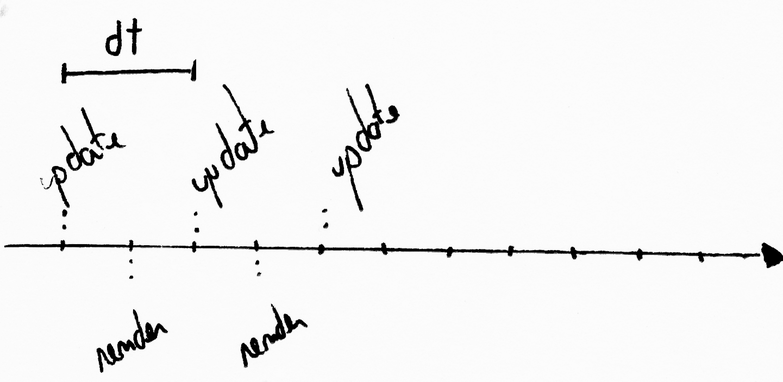
\includegraphics[width=\textwidth]{imagens/ilu2_small.png}
	\caption{Execução do game loop com timestep fixo ao longo do tempo}
\end{figure}

\subsection{Timestep variável}
Para que a taxa de atualização $\Delta t$ seja dinâmica ao invés de fixa, ela precisa ser independente do FPS. Isso é possível medindo-se quanto tempo transcorre entre um frame e outro. Dessa forma o game loop fica definido como se segue:

\begin{lstlisting}[caption=Game loop com timestep variável]
private long lastFrame;
private long dt;
		
while(true) {
	long currentFrame = System.nanoTime(); 
	dt = currentFrame - lastFrame;
	lastFrame = currentFrame;
	
	update(dt);
	render();
}
\end{lstlisting}
Esse código é representado pela figura:
\begin{figure}[H]
	\centering
	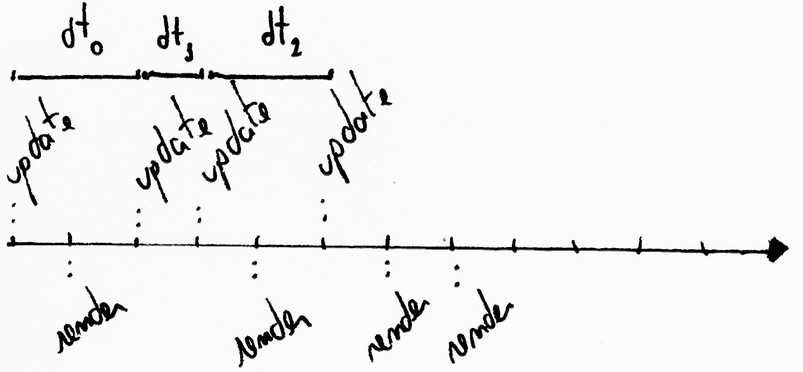
\includegraphics[width=\textwidth]{imagens/ilu3_small.png}
	\caption{Execução do game loop com timestep variável ao longo do tempo}
\end{figure}

Embora tenha-se resolvido o problema anterior de dois computadores com capacidades diferentes de processamento, o sistema ainda não é ideal. A falha está no fato de utilizar o $\Delta t$ anterior ao frame atual. Se o tempo passado entre um frame e outro for muito grande, ou seja, se houver um pico de performance, será avançado um tempo muito grande e um passo do personagem que era para ser $10 pixels$, passa a ser $10px + atraso$. Isso gera um efeito chamado de \textit{stuttering} e é percetível ao jogador, pois atrapalha a fluidez da movimentação. Isso também traz consequências na lógica do programa. Um objeto que deveria percorrer 10 pixels por timestep, ao percorrer mais em um único timestep poderia, por exemplo, estar ignorando uma colisão que iria ocorrer entre o ponto atual e o próximo.
\begin{figure}[H]
	\centering
	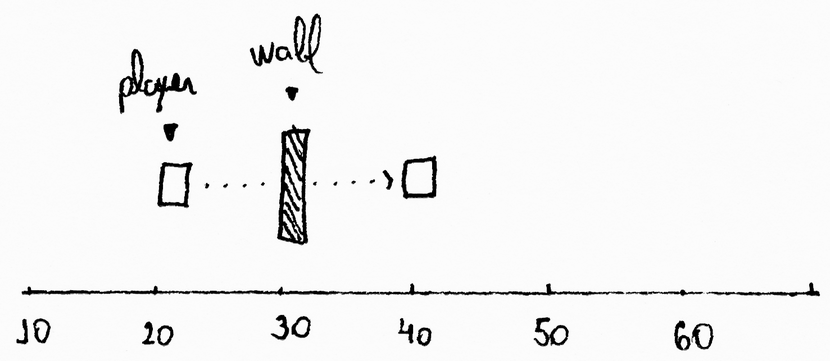
\includegraphics[width=\textwidth]{imagens/ilu4_small.png}
	\caption{Objeto ignorando colisão devido um timestep muito grande}
\end{figure}
 Não só isso, mas um timestep variável traz toda uma complicação com a depuração. Ao introduzir um fator não determinístico no processo, pode ser que seja impossível reproduzir um cenário de bug para efetuar seu diagnóstico e correção. 

\subsection{Timestep semi-fixo}
Um game loop com timestep semi-fixo tenta trazer o melhor dos dois mundos. Isso é possível usando um $\Delta t$ fixo para cada chamada do método update e, quando o sistema demorar mais que o $\Delta t$ fixado, faz-se a recuperação do mesmo chamando o método \texttt{update} quantas vezes necessário.
Isso é fácil visualizar quando demonstrado em código:

\begin{lstlisting}[caption={Game Loop com timestep semi-fixo}]
private long lastFrame;
private long accumulator = 0;
private long dt;
public static final long ONE_SECOND_IN_NANOSECONDS = 10^9;
public static final long STEPS_PER_SECOND = 30;
public static final long FIXED_DT = ONE_SECOND_IN_NANO/STEPS_PER_SECOND;
			
while(true) {
	long currentFrame = System.nanoTime(); 
	dt = currentFrame - lastFrame;
	lastFrame = currentFrame;
	accumulator += dt;
	
	while (accumulator >= FIXED_DT){
    	update(dt);
    	accumulator -= FIXED_DT;
 	 }
 			 
	render();
}
\end{lstlisting}

É importante ter cuidado com o valor escolhido para o \texttt{FIXED_DT} (timestep). Se o timestep for menor que o tempo que se leva para processar o método \texttt{update} o sistema nunca irá recuperar seu atraso, tendo um acumulador que sempre cresce e nunca fica próximo de zerar \cite{GameProgrammingPatterns}.
O sistema de timestep semi-fixo é demonstrado pela ilustração:
\begin{figure}[H]
	\centering
	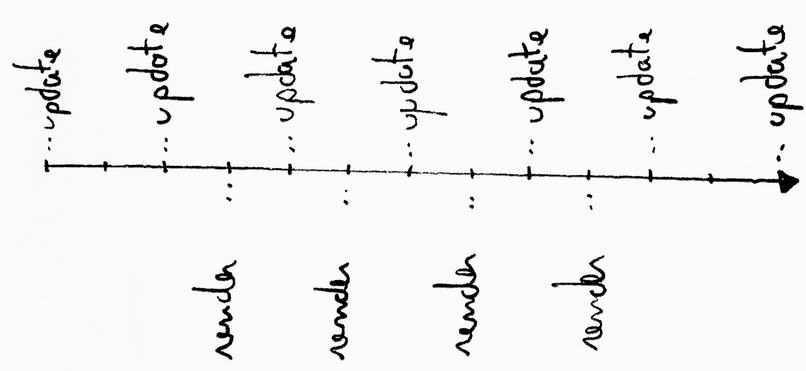
\includegraphics[width=\textwidth]{imagens/ilu6_small.png}
	\caption{Execução do game loop com timestep semi-fixo ao longo do tempo}
\end{figure}
O problema em que o processamento do método update é maior que o $\Delta t$ é mostrado na figura seguinte. Note que o valor de $dt_0$ é maior que o $\Delta t$ fixado e o sistema só tende a piorar ao longo do tempo, acumulando cada vez mais atraso nos valores de $dt$ e nunca se recuperando.
\begin{figure}[H]
	\centering
	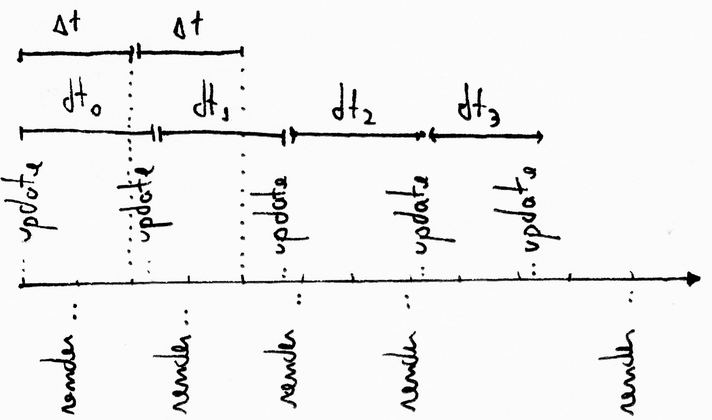
\includegraphics[width=\textwidth]{imagens/ilu8_small.png}
	\caption{Método \texttt{update} com tempo de processamento maior que o $\Delta t$}
\end{figure}
 
\section{Sistema de renderização}
É neste sistema que todos os objetos visíveis na tela são desenhados. Esse sistema é executado diversas vezes e em rápida sucessão durante um segundo através do método \texttt{render}, criando uma ilusão de movimento. Esse processo se inicia no processador e termina na placa gráfica acontecendo quantas vezes a máquina conseguir ou quantas vezes o usuário desejar configurar. Os valores mais comuns para fixar o FPS são atrelados à frequência do monitor que, atualmente, variam de 30 Hz até 144 Hz e para todos os efeitos Hertz é uma medida equivalente ao FPS \cite{GameEngineArchitecture}.

\subsection{Interpolação Linear} 
Com o timestep definido ainda é necessário mais um procedimento para que o sistema renderize objetos em movimento de forma suave. O efeito de \textit{stuttering} pode ser causado tanto pelo aspecto lógico, através dos picos de performance, quanto pelo simples fato de que não se possui total controle sobre como o SO gerencia a aplicação. Não é possível garantir uma taxa de atualização e renderização intercalada e perfeita. Haverá momentos que depois de um único \texttt{update} o método \texttt{render} será chamado várias vezes se processado em um tempo menor que o $\Delta t$ e, sem nenhum tratamento, este efeito também causa \textit{stuttering}. Ao chamar o método \texttt{render} consecutivamente e não atualizar a posição do objeto em cada chamada, o usuário tem a impressão de um sistema engasgado com movimento não fluído.
Para resolver este último problema é necessário realizar uma interpolação linear entre a posição anterior e atual do objeto, tornando seu movimento suave. Esse efeito pode ser visualizado nas figuras \ref{fig:renderSemInterpolacao} e \ref{fig:renderComInterpolacao} onde um objeto move-se 10 pixels por segundo. Na primeira figura a função \texttt{render} é chamada sem nenhum tratamento e portanto renderiza o objeto no mesmo lugar até que sua posição seja atualizada no próximo \texttt{update}. Já na segunda figura, é renderizada a interpolação da posição desse objeto, tornando seu movimento muito mais suave para o usuário.
\begin{figure}[H]
	\centering
	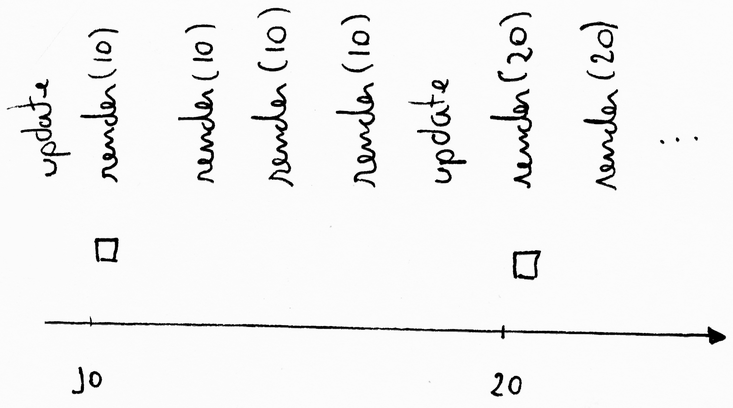
\includegraphics[width=\textwidth]{imagens/ilu7_small.png}
	\caption{Renderização sem interpolação
	\label{fig:renderSemInterpolacao}}
\end{figure}
\begin{figure}[H]
	\centering
	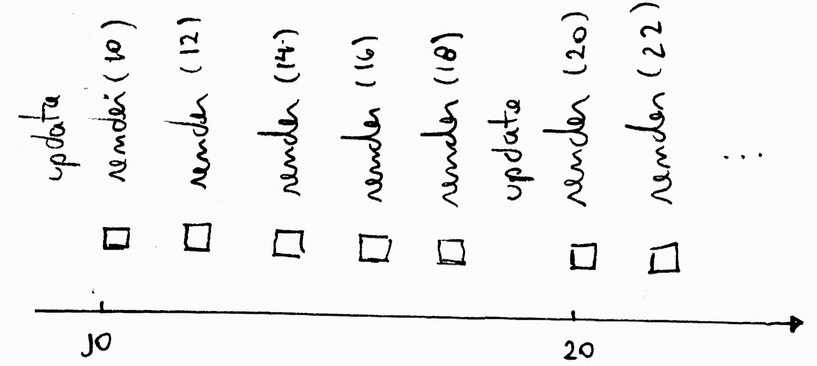
\includegraphics[width=\textwidth]{imagens/ilu5_small.png}
	\caption{Renderização sem interpolação
	\label{fig:renderComInterpolacao}}
\end{figure}

\noindent
O código final do game loop, para um sistema com timestep semi-fixo e com interpolação linear fica como se segue:
\begin{lstlisting}[caption=Game Loop com timestep semi-fixo e interpolação linear]
		long lastFrame;
		long accumulator = 0;
		long dt;
		public static final long ONE_SECOND_IN_NANOSECONDS = 10^9;
		public static final long STEPS_PER_SECOND = 30;
		public static final long FIXED_DT = ONE_SECOND_IN_NANO/STEPS_PER_SECOND;
		
		
		while(true) {
			long currentFrame = System.nanoTime(); 
			dt = currentFrame - lastFrame;
			lastFrame = currentFrame;
			accumulator += dt;
	
			while (accumulator >= FIXED_DT){
    			update(dt);
    			accumulator -= FIXED_DT;
 			 }
 			 
			long interpolationFactor = accumulator / FIXED_DT; 			 
 			 
			render(interpolationFactor);
		}
\end{lstlisting}
Dentro da função \texttt{render} o fator de interpolação é utilizado na seguinte fórmula para obter a posição onde o objeto deve ser renderizado:

\begin{quote}
$renderPosition$ = $currentPosition * interpolationFactor$ + $previousPosition * (1 - interpolationFactor)$
\end{quote}

\section{API gráfica OpenGL}
OpenGL é a API encarregada da comunicação com a GPU. Através dela são realizadas todas as chamadas de função responsáveis por desenhar objetos na tela. Cada Engine deve utilizar uma API dependendo da plataforma na qual o produto final será disponibilizado. Por exemplo, para um sistema mobile existe a API OpenGL ES, para Windows tem-se a OpenGL, DirectX etc. De certa forma, as APIs gráficas compõem essencialmente o sistema de renderização.  

\subsection{Core-profile e Immediate mode}
Immediate mode (legado) é o modo antigo de se operar com OpenGL e foi depreciado em 2008 com o lançamento da versão 3.0 \cite{OpenGLHistory}. Hoje ele é substituído pelo modo \textit{Core-profile}. No modo antigo as funções eram mais fáceis de usar, com muitas funcionalidades já abstraídas pela API. Entretanto, por serem funções abstraídas elas forneciam uma menor flexibilidade de controle sobre como o OpenGL  operava e eram também ineficientes~\cite{LearnOpenGL}. Com o passar do tempo e uma demanda dos desenvolvedores por maior flexibilidade a API foi depreciada e substituída pelo modo \textit{Core-profile}, em que tem-se muito mais controle sobre como o OpenGL opera. Entretanto, isso vem ao custo de uma maior curva de aprendizagem e complexidade de implementação.

\subsection{State Machine}
O OpenGL funciona como uma grande máquina de estados, possuindo uma enorme coleção de variáveis que definem como  operar no estado vigente. Chamam-se as funções para configurar o estado atual, passar dados (coordenadas geográficas, cores e outras informações) ou alterar modos de operação. Um desses estados é o \textit{rendering state} cujo divisão é feita em várias categorias como: \textit{color}, \textit{texturing}, \textit{lighting} e assim por diante. O \textit{rendering state} é manipulado pelas funções \texttt{glEnable(feature)} e \texttt{glDisable(feature)} que recebem como argumento um \texttt{enum} indicando qual o atributo que se deseja habilitar.

\subsection{Hello window}
A primeira etapa necessária para usar o OpenGL é criar um contexto e uma janela onde renderizar. O processo de criação da janela é específico de cada SO e faz-se necessário o uso de outra API para abstrair esse passo. A biblioteca a ser utilizada será a \texttt{GLFW}. O código a seguir demonstra esse processo:
\begin{lstlisting}[caption=Inicialização da janela e contexto OpenGL]
public class Window {
	private int width;
	private int height;
	private Vec2 size;
	private String name;
	private long id;
	
	public Window(int width, int height, String name) {
		this.width = width;
		this.height = height;
		this.name = name;
		size = new Vec2(width,height);
	}
	
	public void init() {
		if (!glfwInit()) 
			System.err.println("Could not initialize GLFW.");

		glfwWindowHint(GLFW_CONTEXT_VERSION_MAJOR, 3);
		glfwWindowHint(GLFW_CONTEXT_VERSION_MINOR, 3);
		glfwWindowHint(GLFW_OPENGL_PROFILE, GLFW_OPENGL_CORE_PROFILE);
		glfwWindowHint(GLFW_RESIZABLE, GL_FALSE);

		id = glfwCreateWindow(width, height, name,  NULL,  NULL);
		glfwMakeContextCurrent(id);

		glfwSetWindowPos(id, 2000, 60);
		glfwShowWindow(id);
		GL.createCapabilities();
		glfwSwapInterval(1); //VSYNC

		glViewport(0,0, width, height);
		glEnable(GL_CULL_FACE);
		glEnable(GL_BLEND);
		glBlendFunc(GL_SRC_ALPHA, GL_ONE_MINUS_SRC_ALPHA);
	}
}
\end{lstlisting}
Primeiramente inicia-se o GLFW através da chamada \texttt{glfwInit()}. Em seguida usa-se a função \texttt{glfwWindowHint(hint, value)} para adicionar atributos a janela, sendo o primeiro argumento o nome do atributo (de tipo \texttt{enum}) e o segundo argumento o valor que se deseja atribuir. No exemplo definido para a função \texttt{init} acima, foram inseridos os atributos \texttt{GLFW_CONTEXT_VERSION_MAJOR} e  \texttt{GLFW_CONTEXT_VERSION_MINOR} indicando qual a versão mínima para rodar a aplicação. Essa versão é representada no formato [MAJOR].[MINOR] e, portanto, neste cenário a versão é 3.3. O atributo \texttt{GLFW_OPENGL_PROFILE} altera entre o modo core profile e immediate mode (legado). Cria-se então a janela com o método \texttt{glfwCreateWindow(width, height, title, monitor, share)} e usa-se o id retornado para torná-lo contexto vigente com
\linebreak \texttt{glfwMakeContextCurrent(id)}. A função \texttt{glfwShowWindow(id)} é chamada para tornar essa janela visível ao usuário. Para utilizar o OpenGL e criar seu contexto é necessário chamar \texttt{GL.createCapabilities}. A partir deste ponto o OpenGL pode ser utilizado normalmente. A função \texttt{glViewport(0,0, width, height)} define o tamanho do viewport ou, simplesmente, o tamanho da área de renderização e é geralmente usado como tendo o mesmo tamanho da janela.

\subsection{OpenGL Pipeline}
No intuito de desenhar objetos na janela, é necessário abordar dois elementos do OpenGL: \textit{buffer objects} e \textit{pipeline}. Os \textit{buffer objects} são estruturas responsáveis por transmitir e encapsular os dados a serem enviados para a GPU. Existem 9 tipos de objetos e estes são divididos em duas categorias~\cite{OpenGLObject}:

\begin{enumerate}
\item \textbf{Regular objects}: objetos dessa categoria contêm dados.
\begin{itemize}
\item Buffer object
\item RenderBuffer object
\item Texture object
\item Query object
\item Sampler object
\end{itemize}
\item \textbf{Container objects}:  objetos dessa categoria servem apenas de containers para transportar os elementos da lista anterior (\textit{regular objects}). 
\begin{itemize}
\item Framebuffer object
\item Vertex Array object
\item Transform Feedback object
\item Program pipeline object
\end{itemize}
\end{enumerate}

Neste primeiro momento será abordado o \textit{Vertex Buffer Object} (VBO) e \textit{Vertex Array Object} (VAO). A fim de desenhar um objeto na tela faz-se necessário enviar a GPU os vértices que o compõem. O \textit{pipeline} recebe como entrada uma série de vértices, os processa e transforma em pixels 2D na tela \cite{LearnOpenGL}. Cada etapa do \textit{pipeline} recebe como entrada a saída da etapa anterior.

As etapas customizáveis do \textit{pipeline} são processadas por pequenos programas chamados \textit{shaders}. Esses programas são escritos em GLSL pelo desenvolvedor da aplicação e ficam alojados na GPU, sendo altamente paralelizáveis e especializados. A seguir tem-se uma representação simplificada do processo que ocorre no pipeline para desenhar um pequeno triângulo.

\begin{figure}[H]
	\centering
	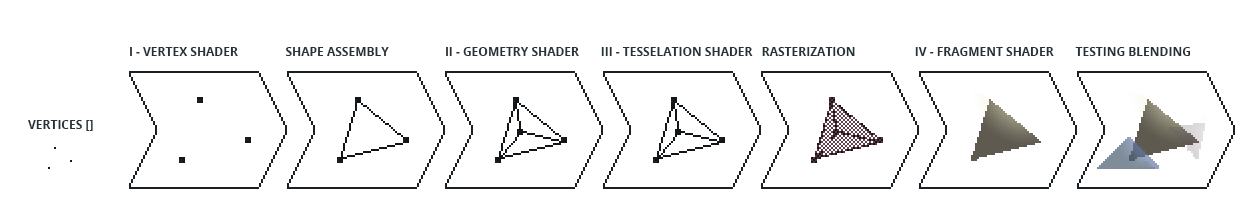
\includegraphics[width=\textwidth]{imagens/openglpipeline.png}
	\caption{Etapas do pipeline  \label{fig:pipeline}}
\end{figure}

Na etapa I o \textit{vertex shader} é responsável, principalmente, por receber um único vértice e transformar sua coordenada cartesiana de um sistema para outro. Por exemplo, as coordenadas finais desse objeto vão mudar conforme a câmera se movimenta no espaço. É também necessário converter a posição local do objeto para a sua posição global no ambiente. Esses e outros processos serão melhor abordados no capítulo sobre Sistemas de Coordenadas.

Na etapa do \textit{shape assembly} o OpenGL monta todos os vértices recebidos como entrada na primitiva selecionada para renderização. São algumas delas: \textit{GL_POINTS}, \textit{GL_LINES} e \textit{GL_TRIANGLES}.

A etapa do \textit{geometry shader} recebe como entrada a primitiva de saída do \textit{shape assembly}. A partir desses vértices o \textit{geometry shader} é capaz de gerar novos vértices e formar novas primitivas. No exemplo da Figura \ref{fig:pipeline} ele recebe um triângulo e cria um novo vértice no centro, resultando em 3 sub-triângulos.

O \textit{tesselation shader} é altamente especializado em subdividir uma primitiva em outras muito menores. Essa função é útil para, por exemplo, detalhar objetos mais próximos da tela e generalizar objetos mais distantes reduzindo sua quantidade de vértices.

A etapa de \textit{rasterization} processa a saída do \textit{tesselation shader} e converte todas essas informações em coordenadas 2D na tela ou, simplesmente, em pixels na tela. Esses pixels são então repassados como fragmentos para o \textit{fragment shader}.

Na penúltima etapa do pipeline, o \textit{fragment shader} processa todos os fragmentos para dar aos pixels sua cor final. É neste estágio que todos os efeitos visuais são aplicados como, por exemplo, a iluminação.

Por fim, no último estágio é aplicado o \textit{blending} e  outros testes. \textit{Blending} nada mais é do que calcular o quanto a transparência de um objeto afeta outro. No exemplo da Figura \ref{fig:pipeline} isso é representado pelos dois triângulos menores que afetam a cor final do triângulo maior aonde estes se sobrepõem. Neste estágio também são realizados os testes de \textit{depth} e \textit{stencil}.

\subsection{Vertex Array Object e Vertex Buffer Object}
Todo objeto no OpenGL é manipulado através de seu ID. Portanto, faz-se necessário gerar o ID do VAO e VBO chamando as funções \texttt{glGenVertexArrays()} e \linebreak \texttt{glGenBuffers()}. Após gerados os IDs vincula-se esse \textit{data object} como o vigente através da função \texttt{glBindBuffer}\texttt{(type, id)} e insere-se os dados nele através da função \texttt{glBufferData(type, data, draw_type)}. Para o \textit{object container} o processo é similar. Vincula-se o VAO com \texttt{glBindVertexArray(id)} e habilita-se a localização do atributo do vértice no \textit{vertex shader} através da função \texttt{glEnableVertexAttribArray(index)}. Por fim, configura-se como cada vértice deve ser interpretado, nesta situação como um bloco de 4 floats, sendo 2 deles as posições $x$ e $y$ do objeto e os dois últimos a posição $x$ e $y$ da textura que compõem esse objeto. Essa configuração é feita pela função \texttt{glVertexAttribPointer(index, size, type, normalized, stride, pointer)}.

\begin{lstlisting}[caption=Inicialização do VBO e VAO]
private void init() {
	float vertices [] = {
			//Pos	//Texture
			0,	1,	0,	1f,
			1,	0,	1f,	0,
			0,	0,	0,	0,
			
			0,	1,	0,	1f,
			1,	1,	1f,	1f,
			1,	0,	1f,	0
	};
	
	int quadVAO = glGenVertexArrays();
	int VBO = glGenBuffers();
	
	glBindBuffer(GL_ARRAY_BUFFER, VBO);
	glBufferData(GL_ARRAY_BUFFER, BufferUtilities.createFloatBuffer(getVertices(3)), GL_STATIC_DRAW); 
	
	glBindVertexArray(quadVAO);
	glEnableVertexAttribArray(0);
	glVertexAttribPointer(0, 4, GL_FLOAT, false, Float.BYTES * 4, 0);
	
	glBindBuffer(GL_ARRAY_BUFFER, 0);
	glBindVertexArray(0);
}
\end{lstlisting}

A variável \texttt{vertices} contém os vértices no espaço local do objeto. Essas coordenadas são então posteriormente processadas no vertex shader e transformadas em coordenadas globais.
\begin{figure}[H]
	\centering
	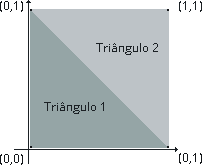
\includegraphics[width=24em]{imagens/tringulosCompondoQuad.png}
	\caption{Dois triângulos em coordenadas locais normalizadas que juntos formam um quadrado}
\end{figure}

\subsection{OpenGL Shading Language (GLSL)}
???

\subsection{Vertex e Fragment shader}
Após a geração do objeto, configuração e posterior transferência dos dados para a GPU, pode-se iniciar o processo de manipulação desses dados no \textit{shader}. Como ilustrado na Figura~\ref{fig:pipeline}, o primeiro shader do pipeline é o \textit{vertex shader}. Todo código escrito no shader é iniciado com a versão do OpenGL. Neste caso, a versão utilizada é a 3.3 e o modo, que deve ser explicitamente citado, é o modo \textit{core profile}.
O index layout, onde o dado é recebido no shader, para este exemplo é 0 e usa o formato de um vetor de 4 floats. Dessa forma a primeira parte do código fica:
\begin{lstlisting}[caption=Vertex shader header]
#version 330 core
layout (location = 0) in vec4 vertex; //xy Obj coord
									  //zw Texture coord
\end{lstlisting}

Definido o cabeçalho agora é necessário dizer quais serão as saídas do shader, ou simplesmente, seu retorno que servirá de entrada para a próxima etapa do pipeline. Isso é feito usando-se a palavra reservada \texttt{out} seguida do tipo e nome da variável. Ainda neste escopo são definidas as variáveis do tipo \texttt{uniform}, que funcionam como variáveis globais e podem ser acessadas em qualquer shader. Em seguida declara-se a função main, responsável pela manipulação destes dados.

 \begin{lstlisting}[caption=Vertex shader simples]
#version 330 core
layout (location = 0) in vec4 vertex; //xy position
									 //zw Tex coord

out vec2 TexCoords;

uniform mat4 model;
uniform mat4 projection;
uniform mat4 camera;

uniform vec2 flip;

void main(){
	TexCoords = vertex.zw;
	gl_Position = projection * camera * model *  vec4(vertex.xy, 0.0 , 1.0);
}
\end{lstlisting}

Esse shader recebe um vetor de 4 floats contendo as coordenadas $x$ e $y$ do objeto e as coordenadas $z$ e $w$ da textura. As coordenadas da textura são passadas adiante para o fragment shader através da variável \texttt{TexCoords} e as coordenadas do vértice são multiplicadas pelas matrizes de projeção, câmera e modelo para obter as coordenadas globais. O resultado dessa multiplicação é armazenado na variável global do openGL chamada \texttt{gl_Position}.

A próxima etapa a ser abordada é a do fragment shader. Para a construção desse primeiro exemplo a única manipulação que será feita nos fragmentos é a renderização da textura. Com a entrada da etapa anterior (vertex shader) extrai-se da textura contida na variável \texttt{image} a fatia desejada usando as coordenadas em TexCoords (linha 5). Esse resultado é então enviado para a última etapa usando-se a variável \texttt{out vec4 color}.

 \begin{lstlisting}[caption=Fragment shader simples]
#version 330 core
in vec2 TexCoords;
out vec4 color;

uniform sampler2D image;

void main(){
	vec4 imgTex =  texture(image, TexCoords).xyzw;
	color = imgTex;
}
\end{lstlisting}

\begin{figure}[H]
	\centering
	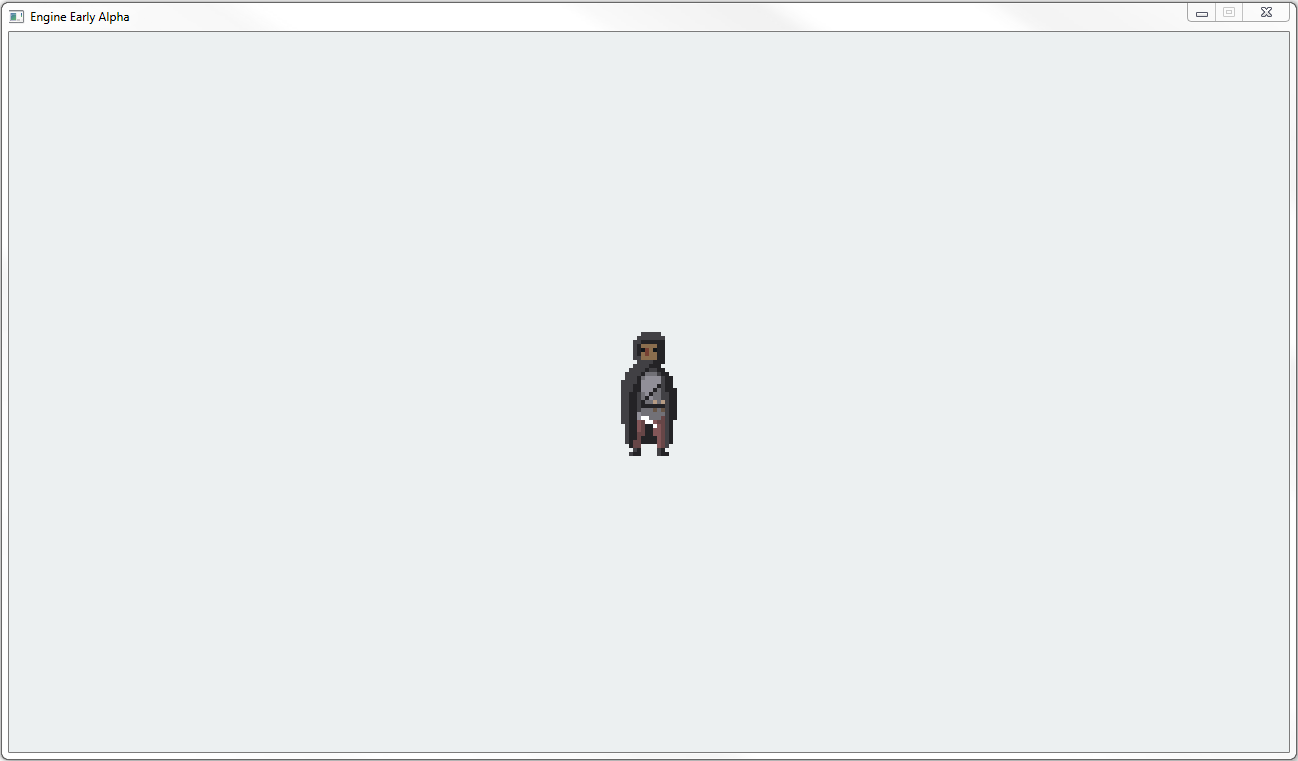
\includegraphics[width=\textwidth]{imagens/helloShader.png}
	\caption{Resultado obtido com dois shaders simples}
\end{figure}

\subsection{Compilando o shader em um programa}
Com o código dos shaders salvos em arquivo é necessário compilá-los e envia-los a GPU antes de poderem ser efetivamente usados. Assim como qualquer objeto no OpenGL o primeiro passo é gerar um ID para referenciá-lo. Esse processo é feito chamando \texttt{glCreateShader(type)}. Os tipos possíveis de shader são aqueles demonstrados e numerados de I a IV na figura \ref{fig:pipeline}. Portanto, os valores possíveis são: \texttt{GL_COMPUTE_SHADER},  \texttt{GL_VERTEX_SHADER},  \texttt{GL_TESS_CONTROL_SHADER},\linebreak  \texttt{GL_TESS_EVALUATION_SHADER},  \texttt{GL_GEOMETRY_SHADER}, e  \texttt{GL_FRAGMENT_SHADER}~\cite{openGLShaderCompilation}. Com o objeto criado atribui-se o código ao objeto e o mesmo é compilado a partir das funções \texttt{glShaderSource(id, code)} e \texttt{glCompileShader(id)}. Para checar se a compilação foi realizada com sucesso chama-se a função \texttt{glGetShaderi(id, GL_COMPILE_STATUS)}, se o retorno for 0 (FALSE) não houve erros. Caso contrário, a função \texttt{glGetShaderInfoLog(id)} retorna a mensagem de erro, que pode ser posteriormente impressa na tela.

 \begin{lstlisting}[caption=Processo de compilação do shader]
	int vertexShader = glCreateShader(GL_VERTEX_SHADER);
	glShaderSource(vertexShader, vertexSource);
	glCompileShader(vertexShader);
	
	int success = glGetShaderi(vertexShader, GL_COMPILE_STATUS);
			
	if(success==0) {
		String log = glGetShaderInfoLog(object);
		System.err.println(log);
	}
\end{lstlisting}

Tendo os shaders compilados agora é necessário criar um programa. Essa etapa segue um padrão baseado no processo de dois estágios para compile/link usada nos programas escritos em C e C++. O código fonte é primeiro servido ao compilador, produzindo um object file. Para obter o executável final é necessário encadear um ou mais object files juntos. Com o programa criado e os shaders encadeados a ele é possível utilizar todos esses shaders com apenas uma chamada do programa.

 \begin{lstlisting}[caption=Processo de criação e link de um programa]
	int id = glCreateProgram();
	glAttachShader(id, vertexShader);
	glAttachShader(id, fragmentShader);
	glLinkProgram(id);
	
	int success = glGetProgrami(object, GL_LINK_STATUS);
			
	if(success==0) {
		String log = glGetProgramInfoLog(object);
		System.err.println(log);
	}
\end{lstlisting}

Os shaders uma vez encadeados podem ser deletados para liberar espaço usado a função \texttt{glDeleteShader(id)}.

\subsection{Uniforms}

Existem duas formas de se enviar dados para um shader, através dos objects e através das variáveis globais definidas como \texttt{uniform}. Para alocar um valor nessas variáveis é necessário primeiro usar o programa que contém este shader com a função \texttt{glUseProgram(id)} e em seguida usar uma das funções da família \texttt{glUniform...()}. O formato dessas funções é glUniform+quantity+type. Por exemplo, para atribuir um valor a uma váriavel float utiliza-se \texttt{glUniform1f (glGetUniformLocation (programID, variableName), value)}, para um vetor de 3 floats usa-se \texttt{glUniform3f(glGetUniformLocation (programID,variableName), x, y, z)}, para uma matriz 4 por 4  \texttt{glUniformMatrix4fv(glGetUniformLocation (programID,variableName), false, BufferUtilities.createFloatBuffer(m))} e assim por diante.
Dessa forma a classe final do Shader fica:

 \begin{lstlisting}[caption=Shader class]
public class Shader {
	private int id;
	
	public Shader use() {
		glUseProgram(this.id);
		return this;
	}
	public int getId() {
		return id;
	}
	
	/**
	 * Compile all vertex, fragment and geometry source code into a linked program.
	 * Geometry is optional.
	 * 
	 * @param vertexSource
	 * @param fragmentSource
	 * @param geometrySource
	 */
	public void compile(String vertexSource, String fragmentSource, String geometrySource) {
		int vertexShader, geometryShader = 0, fragmentShader;
		
		vertexShader = glCreateShader(GL_VERTEX_SHADER);
		glShaderSource(vertexShader, vertexSource);
		glCompileShader(vertexShader);
		checkCompileErrors(vertexShader, "VERTEX");
		
		fragmentShader = glCreateShader(GL_FRAGMENT_SHADER);
		glShaderSource(fragmentShader, fragmentSource);
		glCompileShader(fragmentShader);
		checkCompileErrors(fragmentShader, "FRAGMENT");
		
		if(geometrySource!=null) {
			geometryShader = glCreateShader(GL_GEOMETRY_SHADER);
			glShaderSource(geometryShader, geometrySource);
			glCompileShader(geometryShader);
			checkCompileErrors(fragmentShader, "GEOMETRY");
		}
		
		id = glCreateProgram();
		glAttachShader(id, vertexShader);
		if(geometrySource!=null)
			glAttachShader(id, geometryShader);
		glAttachShader(id, fragmentShader);
		glLinkProgram(id);
		checkCompileErrors(id, "PROGRAM");
		
		glDeleteShader(vertexShader);
		glDeleteShader(fragmentShader);
		if(geometrySource!=null)
			glDeleteShader(geometryShader);
	}
	
	private void checkCompileErrors(int object, String type) {
		int success;
		String log;
		
		if(type!="PROGRAM") {
			success = glGetShaderi(object, GL_COMPILE_STATUS);
			
			if(success==0) {
				log = glGetShaderInfoLog(object);
				System.err.println(log);
			}
				
		}else {
			success = glGetProgrami(object, GL_LINK_STATUS);
			
			if(success==0) {
				log = glGetProgramInfoLog(object);
				System.err.println(log);
			}
				
		}
	}
	
	public void setFloat(String name, float value) {
		glUniform1f(glGetUniformLocation(id,name), value);
	}
	
	public void setInteger(String name, int value) {
		glUniform1i(glGetUniformLocation(id,name), value);
	}
	
	public void setVec2(String name, float x, float y) {
		glUniform2f(glGetUniformLocation(id,name), x,y);
	}
	
	public void setVec2(String name, Vec2 pos) {
		glUniform2f(glGetUniformLocation(id,name), pos.x, pos.y);
	}
	
	public void setVec3(String name, float x, float y, float z) {
		glUniform3f(glGetUniformLocation(id,name), x,y,z);
	}
	
	public void setVec3(String name, Vec3 pos) {
		glUniform3f(glGetUniformLocation(id,name), pos.x, pos.y, pos.z);
	}
	
	public void setVec4(String name, float x, float y, float z, float w) {
		glUniform4f(glGetUniformLocation(id,name), x, y, z, w);
	}
	
	public void setVec4(String name, Vec4 pos) {
		glUniform4f(glGetUniformLocation(id,name), pos.x, pos.y, pos.z, pos.w);
	}

	public void setMat4(String name, Mat4 m) {
		glUniformMatrix4fv(glGetUniformLocation(id,name), false, BufferUtilities.createFloatBuffer(m));
	}
}
\end{lstlisting}
\section{Renderer}
\subsection{Textura}
Com o shader compilado e encadeado em um programa e os VBO's e VAO's prontos tudo que falta para renderizar a primeira imagem é carregá-la do arquivo e transferí-la para o shader usando uma \textit{texture unit}. Esse processo tem início, como todo objeto no OpenGL, gerando um $id$ via função. Para texturas a função utilizada é \texttt{glGenTextures()}. Em Java utiliza-se a classe \texttt{BufferedImage} para ler a imagem do arquivo e depois passar os pixels em formato de Buffer para o OpenGL.

\begin{lstlisting}[caption=Inicializando uma textura no OpenGL a partir de um BufferedImage]
public class Texture {
	private int id;
	private BufferedImage textureImage;
	private static final int BYTES_PER_PIXEL = 4;
	private int width, height;
	
	public Texture(String path) {
		id = glGenTextures();
		
		try {
			textureImage = ImageIO.read(getClass().getResourceAsStream(path));
			width  = textureImage.getWidth();
			height = textureImage.getHeight();
		} catch (IOException e) {
			e.printStackTrace();
		}
		
		init();
	}
	
	private void init() {
		int[] pixels = new int[textureImage.getWidth() * textureImage.getHeight()];
		textureImage.getRGB(0, 0, textureImage.getWidth(), textureImage.getHeight(), pixels, 0, textureImage.getWidth());
        ByteBuffer buffer = BufferUtilities.createByteBuffer(
        							new byte[textureImage.getWidth() * textureImage.getHeight() * BYTES_PER_PIXEL]
        						); //4 for RGBA, 3 for RGB
        
        for(int y = 0; y < textureImage.getHeight(); y++){
            for(int x = 0; x < textureImage.getWidth(); x++){
                int pixel = pixels[y * textureImage.getWidth() + x];
            
                buffer.put((byte) ((pixel >> 16) & 0xFF));     		// Red component
                buffer.put((byte) ((pixel >> 8) & 0xFF));      		// Green component
                buffer.put((byte) (pixel & 0xFF));              	// Blue component
                buffer.put((byte) ((pixel >> 24) & 0xFF));    		// Alpha component. Only for RGBA
            }
        }

        buffer.flip();

        glBindTexture(GL_TEXTURE_2D, id); //Bind texture ID
        
        //Setup wrap mode
        glTexParameteri(GL_TEXTURE_2D, GL_TEXTURE_WRAP_S, GL12.GL_CLAMP_TO_EDGE);
        glTexParameteri(GL_TEXTURE_2D, GL_TEXTURE_WRAP_T, GL12.GL_CLAMP_TO_EDGE);

        //Setup texture scaling filtering
        glTexParameteri(GL_TEXTURE_2D, GL_TEXTURE_MIN_FILTER, GL_NEAREST); //GL_LINEAR for smooth
        glTexParameteri(GL_TEXTURE_2D, GL_TEXTURE_MAG_FILTER, GL_NEAREST);
        
        //Send texel data to OpenGL
        glTexImage2D(GL_TEXTURE_2D, 0, GL_RGBA8, textureImage.getWidth(), textureImage.getHeight(), 0, GL_RGBA, GL_UNSIGNED_BYTE, buffer);
        
        glBindTexture(GL_TEXTURE_2D, 0); //Unbind texture
        textureImage = null; //'free' BufferedImage
	}
}
\end{lstlisting}

Primeiro cria-se um vetor de inteiros com tamanho da área total da imagem (width*height). Logo em seguida esse vetor é preenchido com os pixels do BufferedImage usando \texttt{textureImage.getRGB(startX, startY, width, height, toArray, offset, scanSize)}. Com todos os pixels da imagem no array \texttt{pixels} basta criar um ByteBuffer usando a função auxiliar \texttt{BufferUtilities.createByteBuffer()}.

\begin{lstlisting}[caption=Função auxiliar createByteBuffer]
public class BufferUtilities {
	public static ByteBuffer createByteBuffer(byte[] array) {
		ByteBuffer result = ByteBuffer.allocateDirect(array.length).order(ByteOrder.nativeOrder());
		result.put(array).flip();
		return result;
	} 
}
\end{lstlisting}

Com o byte buffer alocado a próxima etapa é preenchê-lo com os dados contidos no array \texttt{pixels}. O formato escolhido para essa engine foi o RGBA com canais de 1 byte cada, em que cada canal pode assumir valores entre 0 e 255 ($2^8$). Entretanto, a função \texttt{getRGB()} retorna um espaço de cores no formato ARGB e precisa ser convertido para RGBA antes da inserção no buffer.

\begin{figure}[H]
	\centering
	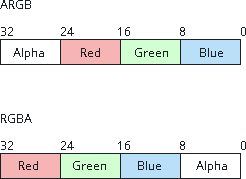
\includegraphics[width=20em]{imagens/sistema_rgba_argb.png}
	\caption{Sistema ARGB e RGBA, ambos com canais de 8 bits (1 byte)}
\end{figure}

Para realizar essa conversão basta aplicar um shift de 24, 16 ou 8 bits conforme o canal e depois aplicar uma máscara de $0x0000FF_{16}$ bits (e.g $11111111_2$) para preservar somente o byte menos significativo. O tamanho do shift depende da posição em que o canal se encontra. A extração do canal verde é exemplificado na figura a seguir.

\begin{figure}[H]
	\centering
	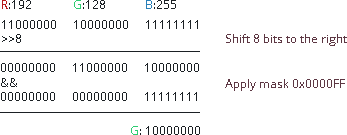
\includegraphics[width=22em]{imagens/extracting_rgb_channel.png}
	\caption{Extração do canal verde em um inteiro de 3 bytes}
\end{figure}

Uma vez que todos os dados foram inseridos no buffer, usa-se \texttt{buffer.flip()}. Antes de qualquer operação na textura vincula-se ela como corrente usando \texttt{glBindTexture(type, id)}. Para este exemplo será utilizado GL_TEXTURE_2D, indicando uma imagem normal em 2D. Em seguida configura-se o modo de \textit{wrapping}. Por padrão, quando as coordenadas de uma textura excedem seu tamanho o openGL as repete com o modo \texttt{GL_REPEAT}. Entretanto, existem 4 modos possíveis: \texttt{GL_REPEAT}, \texttt{GL_MIRRORED_REPEAT}, \texttt{GL_CLAMP_TO_EDGE} e \texttt{GL_CLAMP_TO_BORDER}.
\begin{figure}[H]
	\centering
	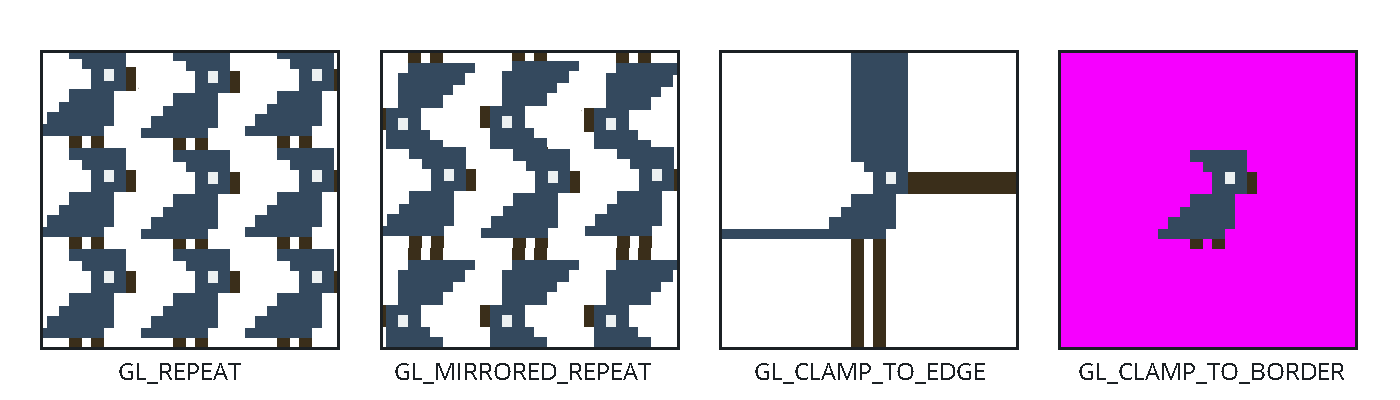
\includegraphics[width=\textwidth]{imagens/wrap_modes.png}
	\caption{Wrap modes}
\end{figure}
Esses modos são configurados através da função \texttt{glTexParameteri(GL_TEXTURE_2D, GL_TEXTURE_WRAP_S, GL12.GL_CLAMP_TO_EDGE}. O segundo argumento indica o eixo para o qual se deseja aplicar a configuração, sendo eles S e T, equivalentes a x e y. Em seguida é escolhido qual a fórmula utilizada para escalonar a imagem. São dois modos possíveis, \texttt{GL_NEAREST} e \texttt{GL_LINEAR}.

O modo GL_NEAREST é o modo default do openGL e opera escolhendo o pixel cujo centro é o mais próximo da coordenada da textura. De uma maneira simples é o modo que ao ampliar a imagem não é aplicado nenhuma suavização, passando uma impressão de imagem serrilhada/pixelada. O exemplo abaixo demonstra esse processo:

O modo GL_LINEAR interpola um valor entre os pixels vizinhos. É o modo que ao ampliar ou diminuir a imagem causa uma impressão de bordas mais suaves.

\begin{figure}[H]
	\centering
	
\includegraphics[width=36em]{imagens/gl_filters.png}
	\caption{Amplicação de 32x usando cada tipo de filtro}
\end{figure}

Esses modos podem ser aplicados distintamente para operações de aumentar ou diminuir a imagem. O atributo responsável por dizer em qual das duas situações o filtro deve ser aplicado é: \texttt{GL_TEXTURE_MAG_FILTER} e \texttt{GL_TEXTURE_MIN_FILTER}. Sendo o primeiro para operações de magnifying (aumento) e o segundo para operações de minifying (diminuir).

Por fim, com todos esses parâmetros configurados envia-se o bytebuffer contendo os dados da imagem propriamente dita para o OpenGL. Isso é feito na função \texttt{glTexImage2D(type, mipmap_level, internal_format, width, height, border, color_format, type, bytebuffer)}

\subsection{Animações}
Uma vez que todo o sistema de shader program e texturas estão montados é possível usá-los para construir componentes mais avançados, como o de animação. Um objeto em animação não é nada mais que uma sequência de frames desenhados em um intervalo de milissegundos, criando ilusão de movimento. É comum a utilização de spritesheets para armazenar todas as imagens em um único arquivo e então recortá-las em pedaços (frames) em tempo de execução.
\begin{figure}[H]
	\centering
	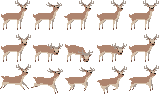
\includegraphics[width=16em]{imagens/spritesheet.png}
	\caption{Spritesheet com frames de 32x32}
\end{figure}
Para que esse recorte seja possível é necessário acrescentar alguns parâmetros ao shader para que este saiba qual pedaço deve ser recortado. Essa tarefa pode ser facilmente realizada alterando as coordenadas locais da textura enviadas através do glAttrib 0 definido anteriormente.
\begin{lstlisting}[caption=Vertex shader com animações]
#version 330 core
layout (location = 0) in vec4 vertex; //xy position
									 //zw Tex coord

out vec2 TexCoords;
out vec3 FragPos;

uniform mat4 model;
uniform mat4 projection;
uniform mat4 camera;
uniform vec4 spriteFrame; 	//xy 	top left point of the spriteFrame
							//zw	width and height

void main(){
	vec2 tCoords = vertex.zw;

	tCoords *= spriteFrame.zw;
	tCoords += spriteFrame.xy;

	TexCoords = tCoords;
	gl_Position = projection * camera * model *  vec4(vertex.xy, 0.0 , 1.0);
	FragPos = vec3(model * vec4(vertex.xy , 0.0, 1.0));
}

\end{lstlisting}

Na variável \texttt{spriteFrame}

\subsection{Z-Ordering}

\subsection{Light}
\subsubsection{Ambient}
\subsubsection{Diffuse}
\subsubsection{Normals}

\chapter{Desenvolvimento do trabalho}
\label{sec:desenv}
\section{Mecânicas}
\subsection{Sistema de caça ativa}
\begin{figure}[H]
	\centering
	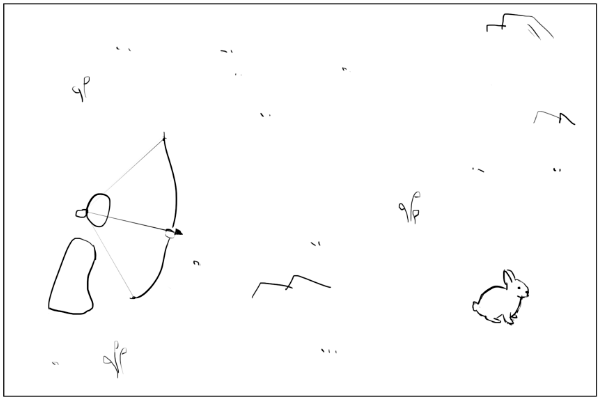
\includegraphics[width=4in]{imagens/mecanica_caca.png}
	\caption{Jogador caçando um coelho com arco e flecha}
\end{figure}
O sistema de caça é dado pelo seguinte fluxo de ações:
\begin{enumerate}  
\item Jogador avista animal em ambiente selvagem 
\item Ao se aproximar o animal pode perceber sua presença. Caso seja notado, a presa irá executar uma animação indicando que está desconfiado.
\item Se o jogador continuar avançando o animal irá tentar fugir 
\item Senão o jogador executa um ataque quando estiver ao alcance 
\end{enumerate}


\subsection{Sistema de armadilhas}
\begin{figure}[H]
	\centering
	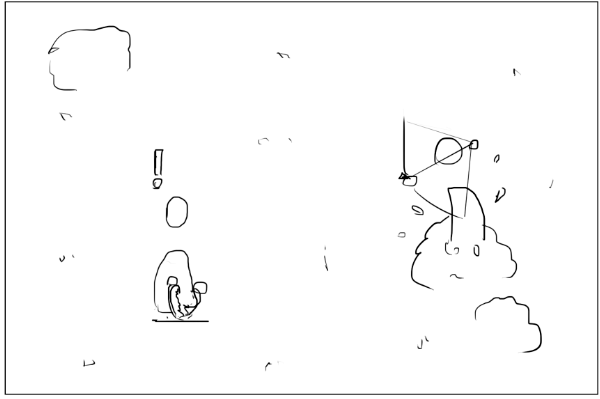
\includegraphics[width=4in]{imagens/mecanica_armadilha.png}
	\caption{Jogador pronto para atacar alvo que ficou preso na armadilha de chão}
\end{figure}
O sistema de armadilhas é dado pelo seguinte fluxo de ações:
\begin{enumerate}  
\item Jogador aciona armadilha no local desejado
\item Qualquer animal ou inimigo pode acionar a armadilha e acionar o seu efeito
\end{enumerate}

\subsection{Sistema de Combate}
O sistema de combate é delimitado pela arma escolhida. Cada arma implica em um estilo
de combate totalmente diferente e só pode ser utilizada ao aprender esse estilo com um
mestre. Os mestres podem ser encontrados aleatoriamente pelo mapa em grandes cidades de 
cada reino.

\subsection{Sistema de apadrinhamento}
Ao atingir um nível significante de reputação o jogador pode tentar ganhar um apadrinhamento de um rei ou lorde. Ganhando assim uma quantia semanal e benefícios como alimento e teto para poder compor suas músicas.

\subsection{Cantar músicas}
\begin{figure}[H]
	\centering
	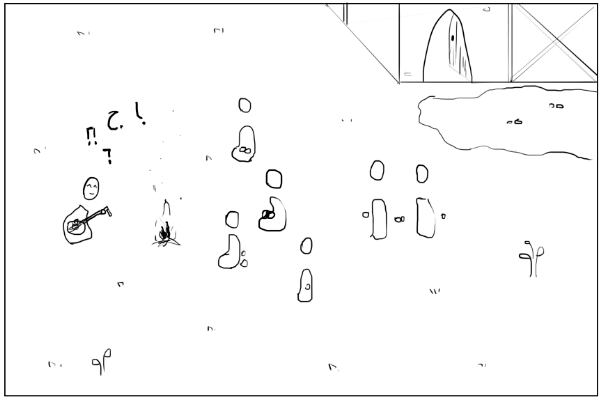
\includegraphics[width=4in]{imagens/mecanica_cantar.png}
	\caption{Jogador cantando em um vilarejo}
\end{figure}
\begin{figure}[H]
	\centering
	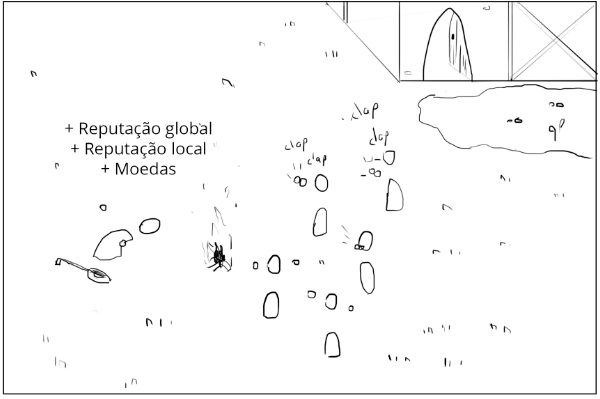
\includegraphics[width=4in]{imagens/mecanica_cantar2.png}
	\caption{Jogador sendo prestigiado após término da música}
\end{figure}
Cada vilarejo ou cidade tem um nível de interesse próprio em determinados instrumentos.
Quanto maior o interesse, maior serão as chances de receber uma boa quantia em ouro
pela apresentação.
As músicas podem ser tocadas em fogueiras que o próprio jogador pode criar em volta da cidade, ou em tavernas, festivais e praças.
\subsection{Compor músicas}
\begin{figure}[H]
	\centering
	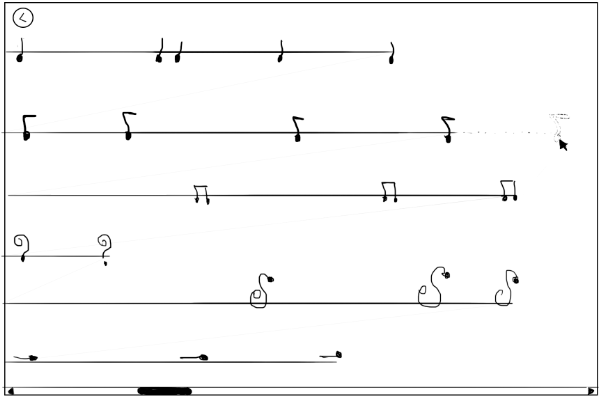
\includegraphics[width=4in]{imagens/mecanica_compormusica.png}
	\caption{Esboço do menu para compor músicas}
\end{figure}
ASD.
\subsection{Contar histórias}
ASD.
\subsection{Compor histórias}
ASD.
\subsection{Atributos dos vilarejos e cidades}
Cada cidade e vilarejo possui os seguintes atributos:
\begin{description}  
\item [Lista de interesses instrumentais] Cada vilarejo tem uma preferência por um instrumento. Quanto maior o interesse, maior a recompensa dada ao tocar músicas com aquele instrumento.
\end{description}

\subsection{Atributos do jogador}
\begin{description}  
\item [Fome] Ao longo do tempo o jogador precisa se alimentar para manter-se vivo. A fome é dividida em três estágios: Sem fome, fome controlável e faminto. Cada um dos estágios é
apresentado ao jogador em forma de uma animação de andar diferente. Quanto mais faminto o personagem está mais lento e curvado ele irá andar, até que ela chegue em zero e culmine na morte do personagem.
\end{description}

\subsection{Domar animais}
Alguns animais podem ser domados através dos instrumentos. Basta cantar próximo a eles então eles serão domados.

% ------------------------------------------
% EXPERIMENTOS E RESULTADOS
\chapter{Experimentos e resultados}
\label{sec:experim}








% ------------------------------------------
% CONCLUSÃO

\chapter{Conclusão}
\label{sec:conclus}







% ----------------------------------------------------------
% ELEMENTOS PÓS-TEXTUAIS


% ----------------------------------------------------------
\postextual

% ----------------------------------------------------------
% Referências bibliográficas
% ------------------------------------------
% REFERÊNCIAS MODELO DA FACOM
\bibliography{referencias}


% OS COMENTÁRIOS ABAIXO É CASO O TRABALHO TENHA ALGUM APÊNDICE
%% Apêndices TCC: só mantenha se for pertinente.
%% ----------------------------------------------------------

% ---
% Inicia os apêndices
% ---
%\begin{apendicesenv}

% Imprime uma página indicando o início dos apêndices
%\partapendices

% ----------------------------------------------------------
%\chapter{Quisque libero justo}
% ----------------------------------------------------------

%\lipsum[50]

% ----------------------------------------------------------
%\chapter{Coisas que fiz e que achei interessante mas não tanto para entrar no corpo do texto}
% ----------------------------------------------------------
%\lipsum[55-57]

%\end{apendicesenv}
% ---


% ----------------------------------------------------------
% Anexos %TCC: so mantenha se pertinente.
% ----------------------------------------------------------

% ---
% Inicia os anexos
% ---
%\begin{anexosenv}

% Imprime uma página indicando o início dos anexos
%\partanexos

% ---
%\chapter{Eu sempre quis aprender latim}
% ---
%\lipsum[30]

% ---
%\chapter{Coisas que eu não fiz mas que achei interessante o suficiente para colocar aqui}
% ---

%\lipsum[31]

% ---
%\chapter{Fusce facilisis lacinia dui}
% ---

%\lipsum[32]

%\end{anexosenv}

%---------------------------------------------------------------------
% INDICE REMISSIVO
%---------------------------------------------------------------------

\printindex



\end{document}